\section{Theorie}
\label{sec:Theorie}
\subsection{Austritsarbeit und Energieverteilung von Elektronen}
Metalle sind kristalline Festkörper. Sie bilden ein Gitter von 
Ionisierten Athomen, welches von nahezu Kräftefrei bewegten Elektronen 
eingehüllt wird. Kräftefrei ist es daher, da im inneren des Metalles das "Gitterpotential"
nahezu konstant ist, sodass sich die Elektronen dort frei bewegen Können. Um Elektronen jedoch 
aus dem Metall zu emmitieren muss eine Austritsarbeit überwunden werden, da das Potential auserhalb 
des Metalls verschieden ist.
\begin{figure}[H]
    \centering
        \centering
        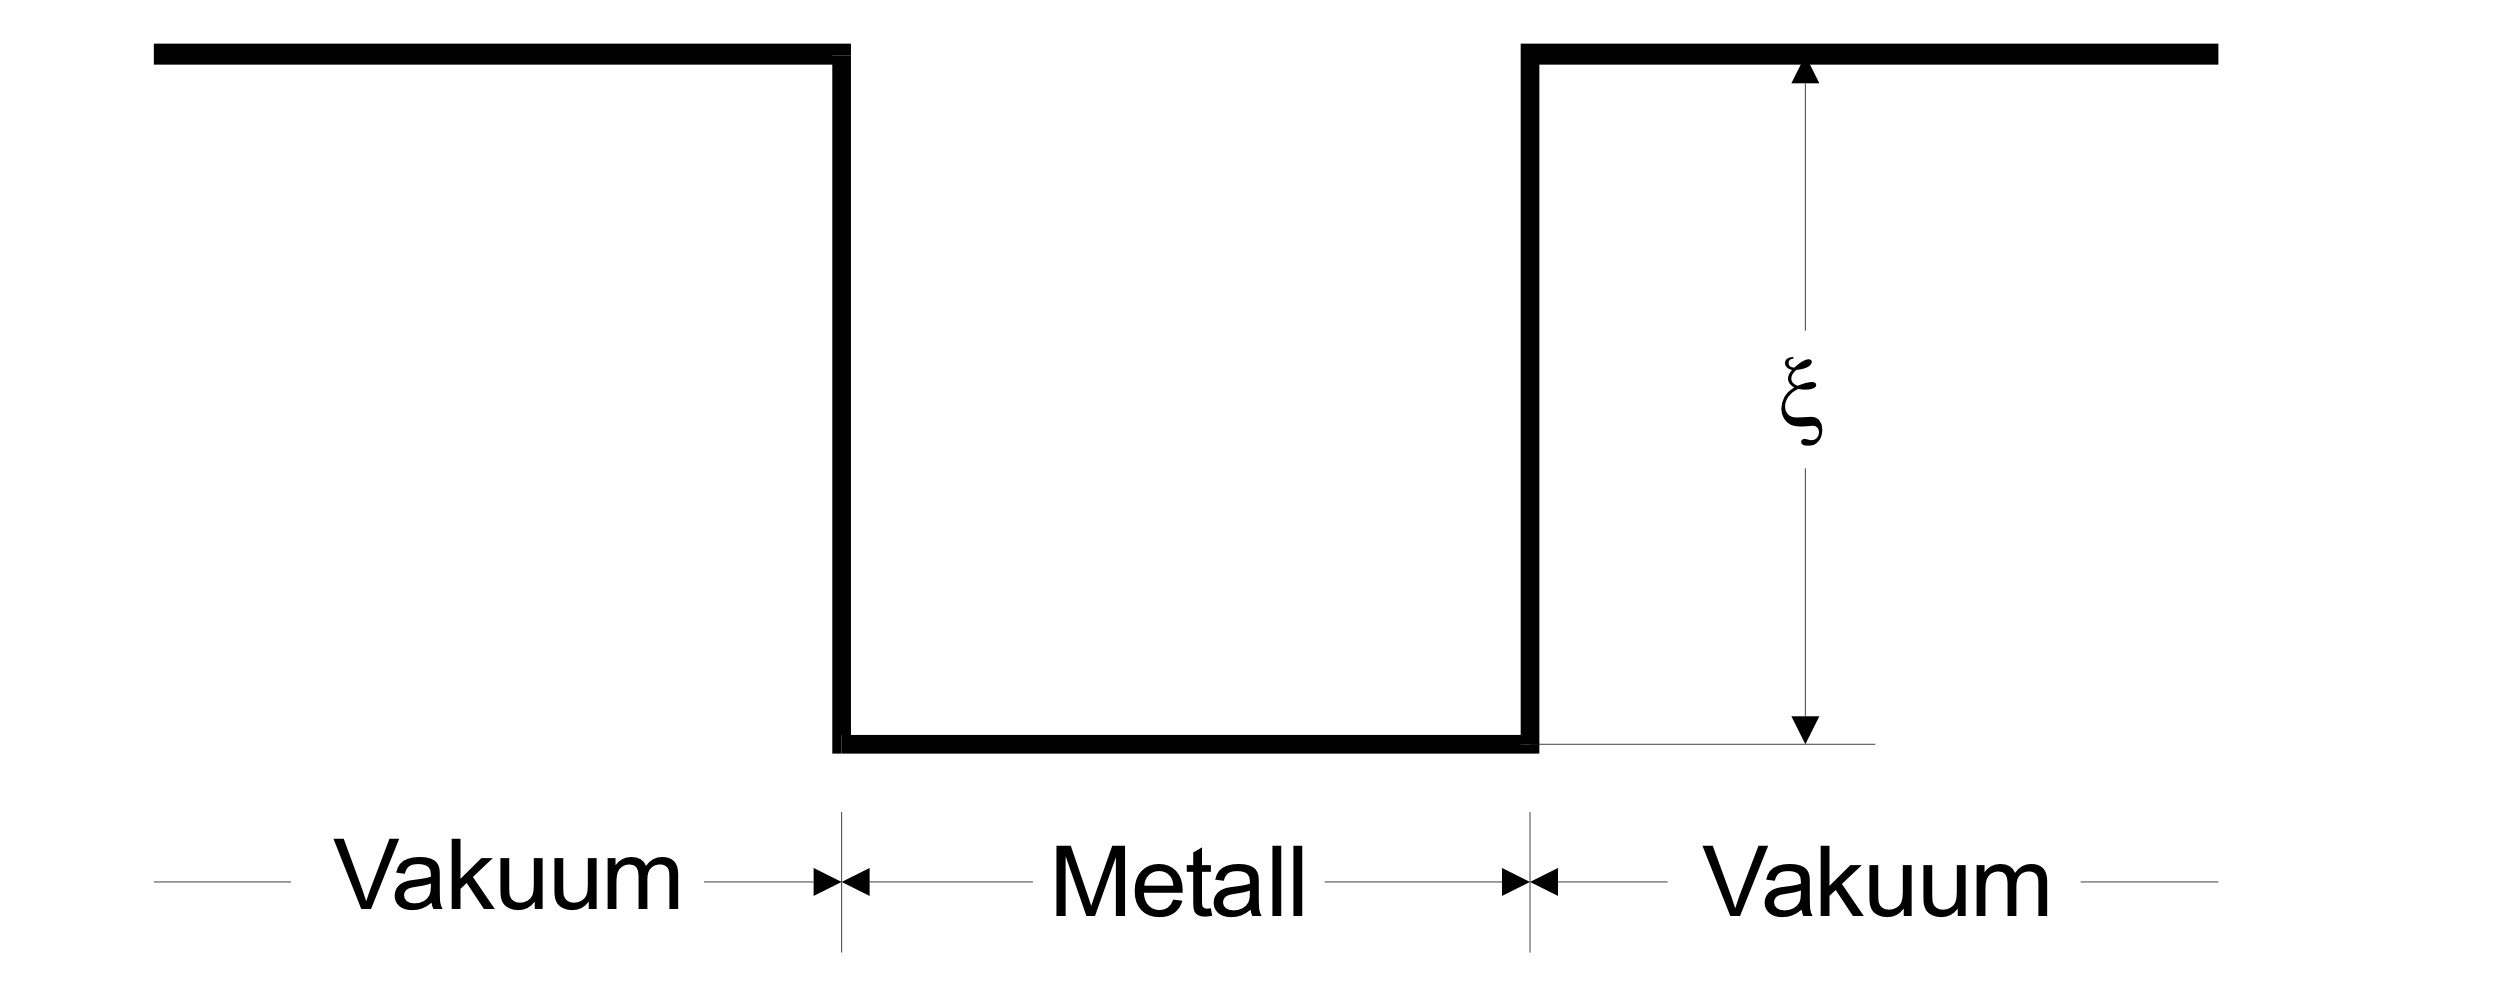
\includegraphics[width=\textwidth]{Bilder/potentialtopf.jpg}
        \caption{Potentialtopf-Modell eines Metalls}
    \hfill
    \label{fig:phasendiagramm}
\end{figure}
Anhand des Potentialtopfmodells lässt sich verdeutlichen, dass die Elektronen eine Austritsarbeit von 
$\exp _0 \Epsilon$ verrichten muss.


\cite{sample}
